\xchapter{相关理论与技术}{Related Theory and Technology}
\xsection{脉冲超宽带雷达感知技术}{Impulse Radio Ultra-Wideband (IR-UWB) Radar Sensing Technology}
超宽带(Ultra-Wideband,UWB)射频是指工作频率带宽超过500MHz的射频信号，由于超宽带射频大多是通过发射极短的无线电脉冲来实现如此高的工作频率带宽，因此也被称为脉冲超宽带(Impulse Radio Ultra-Wideband,IR-UWB)。该射频信号的核心特点在于极宽的频谱带宽和极低的功率谱密度，得益于这两点，超宽带信号可以在短时间内传输大量信息，而不会干扰同一频段的传统窄带和载波传输，因此，超宽带射频已经被广泛地应用于无线通信领域。超宽带射频能够穿透障碍物并且捕获到环境中细微的变化，同时具有极高的时间分辨率，能够实现对目标物体的精确距离测量和运动检测，这些特点让超宽带射频在感知领域也得到应用。与Wi-Fi和RFID等有限带宽的射频模式相比，超宽带射频的超高带宽带来了细粒度的测距分辨率，因此具有精度更高的感知能力；与毫米波和激光这种高频的射频模式相比，超宽带射频具有更小的传播损耗和更强的穿透能力，因此在非视线(Non-Line-of-Sight,NLOS)场景下有着更鲁棒的感知能力；换言之，超宽带射频感知在感知精度和感知鲁棒性上取得了良好的平衡。目前市面上已经有不少基于超宽带射频的商用脉冲超宽带雷达，本文使用的脉冲超宽带雷达为XeThru的X4雷达，该款雷达具有单根发射天线和单根接收天线，中心频率为7.29GHz，带宽为1.4GHz，有不少工作使用该雷达去完成了不同的下游感知任务，例如生命体征监测\cite{zheng2021more, chen2021movi}，空中手写识别\cite{9253617}，人类活动识别\cite{noori2021ultra}，音频振动提取和分离\cite{wang2020uwhear}等。本节后续将详细介绍脉冲超宽带雷达的感知原理以及雷达接收信号的数据结构。
\xsubsection{脉冲超宽带雷达感知原理}{Impulse Radio Ultra-Wideband (IR-UWB) Radar Sensing Theory}
\label{sec:UWB_sense}
脉冲超宽带雷达的调制解调流程如图\ref{fig:baseband}所示，雷达发射被调制在频率为$f_c$的余弦
\begin{figure}[htbp]
    \centering
    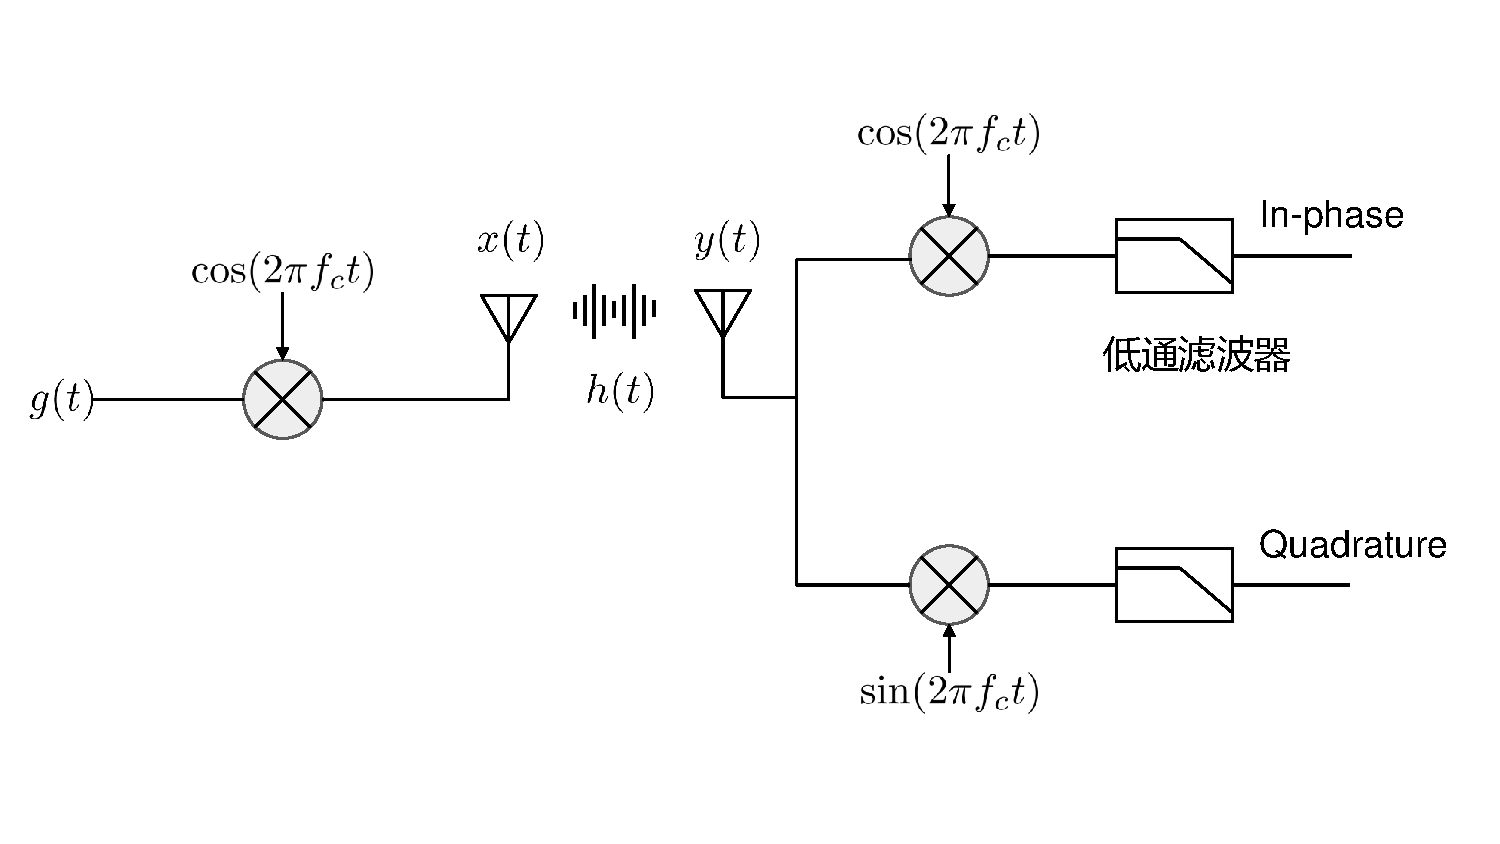
\includegraphics[width=0.7\textwidth]{Figures/baseband.pdf}
    \caption{脉冲超宽带雷达的调制解调流程}
    \label{fig:baseband}
\end{figure}
载波上的高斯脉冲$g(t)$，脉冲信号会以间隔$T_s$周期性地发射，发射信号的数学表示如下：
\begin{equation}
    x(t) = g(t-kT_s)\cos(2\pi f_c(t-kTs))
\end{equation}
高斯脉冲信号$g(t)$可以表示为：
\begin{equation}
    g(t) = V_{tx} exp(-2{\pi}^2{f_B}^2{log}_{10} (e)t^2)
\end{equation}
其中，$f_B$表示-10dB带宽，$V_{tx}$是高斯脉冲的最大幅值。雷达发射的信号被环境中的物体反射并由接收天线接收，通常，发射天线和接收天线会被雷达集成到同一位置上。由于感知范围内存在着不同的反射物体，因此信道响应$h(t)$可以表示为具有不同时延和衰减的$P$条路径的总和：
\begin{equation}
    h(t) = \sum_{p=1}^{P}\alpha_p \delta(t-T_p)
\end{equation}
其中$T_p$是由反射路径距离决定的往返飞行时间，$\delta(t)$表示单位冲激函数，$\alpha_{p}$可以看做是该反射路径固有的反射强度系数，那么接收天线接收到的信号$y(t)$就可以被建模成发射信号与信道脉冲响应的卷积再加上噪声$n(t)$，即：
\begin{equation}
    \begin{aligned}
        y(t) &= x(t) * h(t) + n(t) = \sum_{p=1}^P \alpha_p g(t - kT_s - T_p) \times \cos\left(2\pi f_c (t - kT_s - T_p)\right) + n(t)
    \end{aligned}
\end{equation}
在接收侧，会对接收信号$y(t)$进行下变频操作，具体操作为将$y(t)$在混频器中与载波余弦及正弦信号相乘，再通过低通滤波器(Low-Pass Filter, LPF)，分别得到I路信号(In-phase Signal)和Q路信号（(Quadrature Signal)），对于I路信号，将$y(t)$与余弦载波$\cos(2\pi f_c(t-kT_S))$相乘后，仅考虑余弦部分，有：
\begin{equation}
    \begin{aligned}
        m(t) &= \cos(2\pi f_c (t - kT_S - T_p)) \times \cos(2\pi f_c (t - kT_s)) \\
             &= \frac{1}{2} \left[ \cos \left( 2\pi 2f_c \left( t - kT_s - \frac{T_p}{2} \right) \right) + \cos(2\pi f_c T_p) \right]
    \end{aligned}
\end{equation}
由于$2f_c$频率分量会被低通滤波器滤除，因此只有低频分量$\frac{1}{2}\cos(2\pi f_c T_p)$被留下，因此，在经过下变频和滤波器后的I路信号为:
\begin{equation}
    \begin{aligned}
        y_\text{in-phase}(t) &= LPF[y(t)\cdot cos(2\pi f_c(t-kT_s))] \\
                        &= \frac{1}{2}\sum_{p=1}^{P} \alpha_p g(t-kT_s-T_p)\times\cos(2\pi f_c T_p) +n(t)
    \end{aligned}
\end{equation}
同理，也可以得到Q路信号：
\begin{equation}
    \begin{aligned}
        y_\text{quad}(t) &= LPF[y(t)\cdot\sin(2\pi f_c(t-kT_s))] \\
                    &= \frac{1}{2}\sum_{p=1}^{P} \alpha_p g(t-kT_s-T_p) \times \sin(2\pi f_c T_p) + n(t)
    \end{aligned}
\end{equation}
在数字信号处理领域，I路信号和Q路信号通常一起组成复数信号，那么根据欧拉公式，复数形式的接收信号$y_\text{complex}(t)$可以做如下推导：
\begin{equation}
    \label{equ:y_complex}
    \begin{aligned}
        y_\text{complex}(t) &= y_\text{in-phase}(t) + j\cdot y_\text{quad} \\
                    &= \frac{1}{2}\sum_{p=1}^{P}\alpha_p g(t-kT_s-T_p)\times[\cos(2\pi f_c T_p)+j\cdot \sin(2\pi f_c T_p)] + n(t) \\
                    &= \sum_{p=1}^{P}A_{p}\cdot e^{j\theta_p} + n(t)
    \end{aligned}
\end{equation}
从复数形式的接收信号上，可以很直观地看出，最终的接收信号其实是多个路径的复数反射信号以及噪声的叠加，路径$p$对应的复数反射信号的幅值$A_{p}$为$\frac{1}{2}\alpha_pg(t-kT_s-T_p)$，相位$\theta_p$为$2\pi f_c T_p$。至此，完成了对脉冲超宽带雷达接收信号的数学推导。
\xsubsection{脉冲超宽带雷达数据结构}{Impulse Radio Ultra-Wideband (IR-UWB) Radar Data Structure}
在上一小节中完成了对脉冲超宽带雷达从发射信号到接收信号做了严格的数学推导，下面对雷达接收信号的最终数据结构以及对应的物理意义进行分析。上一小节提到，雷达会以$T_s$为周期持续发射脉冲信号，将从一个脉冲发射开始到该脉冲对应最后一个响应到达结束期间采样到的数据称为一帧(Frame)。在一帧内，时间$t$的概念对应于脉冲信号的飞行时间，因此称之为快时间。雷达连续发射脉冲，所有帧按照时间顺序排序，因此，每一帧可以看做是在更慢时间尺度上的采样，将其称之为慢时间，通常，快时间的尺度为数十皮秒，而慢时间的尺度为数百微秒。如果将连续接收到的帧按时间顺序排列起来，那么可以得到一个二维矩阵，如图\ref{fig:slow_time_fast_time}所示。
\begin{figure}[htbp]
    \centering
    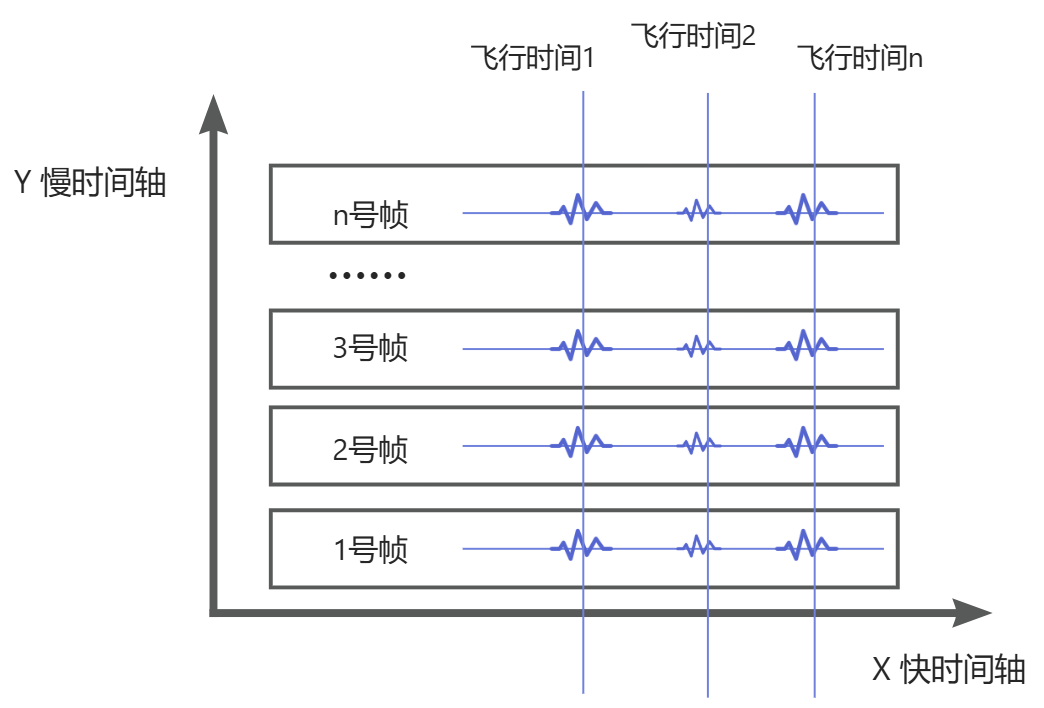
\includegraphics[width=0.5\textwidth]{Figures/slow_time_fast_time.png}
    \caption{二维雷达信号矩阵示意图}
    \label{fig:slow_time_fast_time}
\end{figure}

连续帧沿Y轴（慢时间）排列，在X轴（快时间）上，不同采样点的信号对应着不同时间延迟的反射脉冲响应。由于快时间表示脉冲的往返飞行时间，因此，可以将快时间转换成对应的距离，习惯上，将一个固定的快时间采样点称为一个距离箱。假如待感知物体处于不同的距离下，那么可以通过挑选特定的距离箱来将待感知物体对应的反射信号分离出来，如果物体是动态的，那么可以在连续帧上选择特定距离箱内的信号组成时序信号，从该时序信号中可以提取出物体的运动信息。一个真实的脉冲超宽带雷达的接收数据二维矩阵如图\ref{fig:real_signal}所示，沿着横轴可以切分出单个雷达帧的信号序列，沿着纵轴可以切分出单个距离箱的信号序列。
\begin{figure}[htbp]
    \centering
    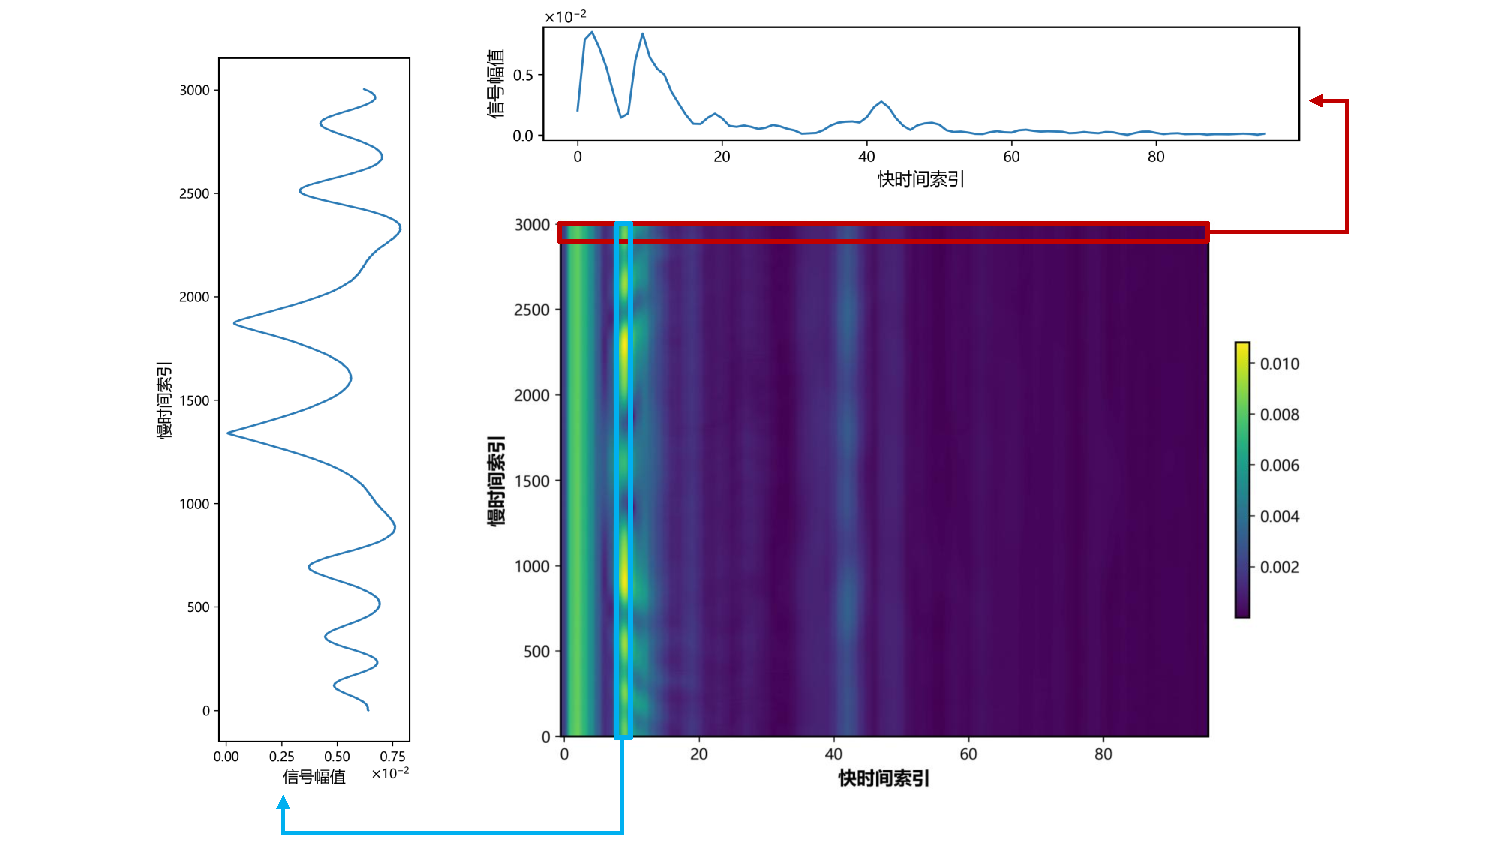
\includegraphics[width=1.0\textwidth]{Figures/signal.pdf}
    \caption{真实雷达信号数据幅值热图}
    \label{fig:real_signal}
\end{figure}

综上所述，脉冲超宽带雷达在一段连续时间内采集的接收信号数据是一个二维的复数矩阵，矩阵的横轴排列着不同的距离箱，纵轴则排列着该距离箱在不同慢时间采样点上的复数信号。当需要感知特定距离上的物体时，可以挑选出物体所在的距离箱，持续跟踪该距离箱上复数信号的时序变化，一般来讲，物体的反射信号会跨越多个距离箱，此时需要同时跟踪多个距离箱的复数信号。
\xsection{迁移学习}{Transfer Learning}
到目前为止，深度学习技术已经取得了显著成功，并在诸多实际应用中展现出卓越的性能，但在应对现实场景中的某些特殊需求时仍存在局限性。传统深度学习范式通常基于两个理想假设：一是存在充足的标注训练样本，二是训练数据与测试数据具有同分布特性。然而在实际应用中，获取充足的训练数据往往面临标注成本高昂、数据采集周期漫长，甚至存在现实条件不可行等困境，本文的基于超宽带虚拟阵列的物体三维点云重建方法是基于深度学习技术的，同样面临着上述训练数据采集标注困难的问题。

迁移学习(Transfer Learning)是上述问题的一个有效解决方法。迁移学习的目的是通过迁移不同但相关的源域中的知识来提高深度学习网络模型在目标域上的表现，通过这种方式，可以减少神经网络模型对大量目标域数据的依赖性。关于迁移学习的一般定义为：迁移学习通过源域$\mathcal{D}_s=(\mathcal{X}_s,P_s(X))$的知识迁移来优化目标域$\mathcal{D}_t=(\mathcal{X}_t,P_t(X))$的任务$\mathcal{T}_t=(\mathcal{Y}_t,f_t)$，其中$\mathcal{D}_s\neq\mathcal{D}_t$或者$\mathcal{T}_s\neq\mathcal{T}_t$，即存在域差异或者存在任务差异。迁移学习可以分为三种主要类型\cite{zhuang2020comprehensive}：直推式迁移学习(Transductive Transfer Learning)、归纳式迁移学习(Inductive Transfer Learning)和无监督迁移学习(Unsupervised Transfer Learning)。这三种类别迁移学习的差异在于源域和目标域标注数据的可见性，当仅有源域的标注数据可见时，该场景被归类为直推式迁移学习；当目标域中的标注数据也可见时，则被归类为归纳式迁移学习；当源域和目标域的标注数据都不可见时，归类为无监督迁移学习。

本文关注归纳式迁移学习，即源域和目标域的标注数据都可见，在这种场景下，迁移学习的训练过程涉及最初在大型数据集上训练基线模型，之后使用较小的目标数据集对其进行微调(Finetune)来达到最佳性能，而并不是直接在相对有限的目标数据集上训练模型，这种训练模式也被称为迁移学习中的“预训练 (Pretrain)-微调 (Finetune)”两阶段学习范式。先前实验的经验证据表明，通过这种两阶段学习，迁移学习能够有效地对抗过拟合，加快训练，并尤其降低了在目标域上训练时所需的数据集大小\cite{hendrycks2019using}。

近年来，迁移学习已经被广泛应用于各领域的深度学习任务中，在医学影像分类领域中，Kathamuthu等人\cite{kathamuthu2023deep}提出了使用迁移学习增强的CNN框架模型，用于使用CT扫描图像检测COVID-19，在最小的数据集上仍能有效检测COVID-19的存在；在机械故障诊断领域，文献\parencite{zhang2023blockchain}提出了一种基于区块链的分散联邦迁移学习方法，有效缓解了单个工业用户数据质量和数量的局限性；在遥感领域，Gomroki等人\cite{gomroki2023stcd}提出了一种半迁移学习方法，成功提升了网络模型在城市土地覆盖变更检测任务上的性能表现；在近年来最火热的大语言模型(Large Language Model,LLM)领域，迁移学习同样应用广泛，低秩适配(Low-rank adaptation,Lora)\cite{hu2022lora}技术作为大模型时代迁移学习的关键技术突破，通过矩阵分解策略在参数效率与知识保留间取得平衡，大大降低了大语言模型微调的训练成本。
\xsubsection{本章小结}{Summary}
本章对本文所使涉及到的相关理论和技术进行了详细的介绍。首先介绍了脉冲超宽带雷达感知技术，其中包括脉冲超宽带雷达感知原理以及对应的雷达数据结构；接着介绍了迁移学习的基本定义，用于解决的问题以及在各个领域的应用情况。
